% Appendix F -- Code examples: Python, Rust (rusty-SUNDIALS) and LeanFlow
% To be placed after \appendix. Every listing is read as is (\lstinputlisting) from code/examples/, and every
% output from code/examples/logs/: these are the files executed on 2026-10-26; nothing is copied by hand.
\chapter{Code examples: Python, Rust (rusty-SUNDIALS) and LeanFlow}\chaptermark{Code examples}\label{appF:chap}

\lstdefinelanguage{Rust}{morekeywords={fn,let,mut,pub,use,struct,impl,for,in,if,else,match,return,move,loop,
  const,type,as,mod,where,true,false,Some,None,Ok,Err,Vec,String,f64,usize,u64,Result,Self,self},
  sensitive=true,morecomment=[l]{//},morestring=[b]"}
\lstdefinestyle{appFcode}{basicstyle=\ttfamily\scriptsize,numbers=left,numberstyle=\tiny\color{gray},
  numbersep=4pt,xleftmargin=1.2em}
\lstdefinestyle{appFlog}{language={},basicstyle=\ttfamily\scriptsize,backgroundcolor=\color{gray!6},
  frame=single,rulecolor=\color{tierX!40},
  literate={/}{{/\allowbreak}}1 {ℕ}{{$\mathbb{N}$}}1 {ℝ}{{$\mathbb{R}$}}1 {→}{{$\to$}}1 {≠}{{$\ne$}}1
  {∀}{{$\forall$}}1 {⁻¹}{{$^{-1}$}}1}
\newcommand{\appFsortie}[1]{\par\noindent\textbf{Actual output} (\texttt{\detokenize{#1}}):%
  \lstinputlisting[style=appFlog]{code/examples/logs/#1}}

Chapters~1 to~5 state theorems and tell how they were verified. This appendix gives the reader the tools to
\emph{redo} the computations that accompany them. It contains twelve examples, spread over the themes of the book.
Each one follows the same plan:
\begin{enumerate}
\item \textbf{the question}, asked before any computation;
\item \textbf{the code}, a short excerpt read directly from the executed file (the line numbers are those of the
file);
\item \textbf{the actual output} of the program, copied by \LaTeX{} from the log of the run;
\item \textbf{a figure}, when it helps to read the numbers;
\item \textbf{an exercise}.
\end{enumerate}

\begin{warnbox}[: what these examples are, and what they are not]
\begin{itemize}
\item A floating-point computation is Tier~X: it illustrates, it tests, it can \emph{refute}, but it never proves.
Only Examples~\ref{appF:ex10} and~\ref{appF:ex11} involve the Lean kernel.
\item Every program runs at least one positive control (a case whose answer is known) and one negative control (a
deliberately false case, which must be refused). It exits with code~1 if a control does not behave as expected. All the
outputs printed here end with \texttt{temoins conformes: True} (``controls as expected'') or
\texttt{controls as expected: true}, except that of Example~\ref{appF:ex11}. That one is the raw output of Lean, which
compiles with exit code~0 even when the planted witness is present; the witness is then read off from
\texttt{\#print axioms}.
\item The code, outputs and figures of this appendix were produced by an AI agent (Claude) under the author's direction,
and checked only by that agent. No human has audited them.
\end{itemize}
\end{warnbox}

\paragraph{Where the files are.} Everything is stored in \texttt{code/examples/}:
\begin{itemize}
\item \texttt{python/}: the Python examples, and \texttt{appF\_style.py}, the common style of the figures;
\item \texttt{rust/}: a byte-for-byte copy of the \texttt{qf-textbook-examples} crate of rusty-SUNDIALS:
\begin{itemize}
\item branch \texttt{textbook2/code-examples-2026-10-26}, branched from \texttt{main} at commit \texttt{7630f7e};
\item commit \texttt{f01b82b730c86ccf05c1f773b11fe0a9b650cc7b};
\end{itemize}
\item \texttt{lean/}: the Lean file of Example~\ref{appF:ex11} and the two certificates generated by LeanFlow in
Example~\ref{appF:ex10};
\item \texttt{logs/}: the outputs printed here; the CSV files written by the Rust binaries are in
\texttt{logs/rust\_out/}.
\end{itemize}

\paragraph{Reproducing.} The Python examples use numpy, scipy, mpmath and matplotlib. They are run with the isolated
interpreter (option \texttt{-I}):
\begin{lstlisting}[language={}]
python -I code/examples/python/f01_poisson.py > code/examples/logs/f01_poisson.txt
\end{lstlisting}
The Rust crate is built in the rusty-SUNDIALS worktree:
\begin{lstlisting}[language={}]
CARGO_TARGET_DIR=~/rusty-target-ar cargo build --release -j 2 --offline -p qf-textbook-examples
~/rusty-target-ar/release/tb_moran_forward code/examples/logs/rust_out
\end{lstlisting}
Before committing, we ran three of the repository's continuous-integration checks, and all three passed:
\begin{itemize}
\item \texttt{cargo fmt --all -- --check};
\item \texttt{cargo clippy --workspace --features experimental -- -D warnings};
\item \texttt{cargo test -p qf-textbook-examples}, with 5 tests out of 5 passing.
\end{itemize}
The full test suite of the workspace was not rerun.

\begin{table}[ht]\centering\small
\caption{The twelve examples. Tier: that of the statement \emph{checked by the program}, not that of the theorem it
illustrates.}\label{appF:tab}
\begin{tabular}{llp{6.1cm}l}\toprule
& language & question & tier\\\midrule
1 & Python & Poisson summation for Gaussians & X\\
2 & Python & energy of the triangular and square lattices (Gaussian, Yukawa, dipolar) & X\\
3 & Python & signs of $(-1)^ng^{(n)}$ with mpmath, and two counterexamples & X\\
4 & Python & exact Wright--Fisher powers, $P^n(i,N)\to i/N$ & X (exact computation)\\
5 & Python & fixation on an isothermal graph and on the star & X (exact computation)\\
6 & Python & phonons and zero-point energy, local maximum & X\\
7 & Rust & CVODE on a stiff ODE, then Moran's Kolmogorov equation & X\\
8 & Rust & relaxation of a small Yukawa crystal & X\\
9 & Rust & the invariants of the $\sigma=3$ shell model & X\\
10 & LeanFlow & certify fixation fractions, reject a planted claim & A (arithmetic)\\
11 & Lean & read and check \lean{ILENE} & A\\
12 & Python & cross-check of CVODE against SciPy & X\\\bottomrule
\end{tabular}
\end{table}

% =====================================================================================================
\section{Example 1 -- Poisson summation for Gaussians}\label{appF:ex1}

\paragraph{The question.} The Poisson summation formula is the engine of Chapters~1 and~3. For a Gaussian in
dimension~1 it reads
\[\sum_{n\in\Z}e^{-\pi a(n+x)^2}=a^{-1/2}\sum_{k\in\Z}e^{-\pi k^2/a}\cos(2\pi kx),\qquad a>0 .\]
For the triangular lattice $\Lat$ of covolume~1, whose dual is a rotation of itself, it gives
$\Theta_\Lat(a)=a^{-1}\Theta_\Lat(1/a)$. Can we see it to within $10^{-15}$? And what is it good for in practice?

\paragraph{The code.} The two sides of the formula, and the theta function of the triangular lattice
($|v|^2=\tfrac{2}{\sqrt3}(m^2+mn+n^2)$):
\lstinputlisting[language=Python,style=appFcode,firstline=23,lastline=38,firstnumber=23]{code/examples/python/f01_poisson.py}
\appFsortie{f01_poisson.txt}

\paragraph{Reading the output.} The two sides agree to machine precision ($10^{-16}$). Without the factor $a^{-1/2}$
(or $a^{-1}$ in dimension~2), the discrepancy is of order~1: this is the negative control. The last line shows the
practical interest of the formula. For $a=0.01$ the Gaussian is very wide: the direct sum needs $n_{\max}=28$ to reach
$10^{-12}$, whereas the dual side is exact from its first term on. This principle, summing on the side where the
function decays fast, is that of Ewald summation.

\begin{figure}[ht]\centering
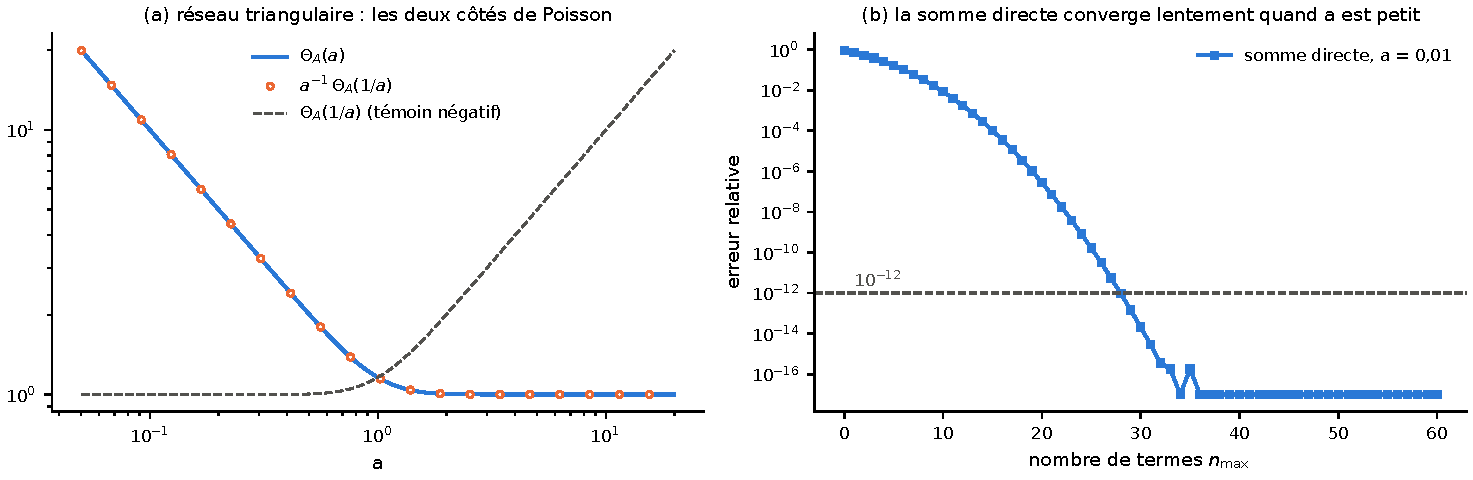
\includegraphics[width=\textwidth]{appF_poisson.pdf}
\caption{Example~1 \tierX. (a) $\Theta_\Lat(a)$ and $a^{-1}\Theta_\Lat(1/a)$ coincide; without the factor $a^{-1}$
(dashed), the curve is wrong. (b) Relative error of the direct sum as a function of the number of terms, for $a=0.01$,
$x=0.3$.}
\label{appF:fig:poisson}
\end{figure}

\begin{exercise}[Example 1]\label{appF:exo1}
(a) Prove the formula in dimension~1 from the Fourier transform of $e^{-\pi ax^2}$, which equals
$a^{-1/2}e^{-\pi\xi^2/a}$. (b) Modify \texttt{theta1} for another even function, $e^{-|x|}$, whose transform is
$2/(1+4\pi^2\xi^2)$, and check the corresponding formula numerically. Why are many more terms needed on the dual side?
\end{exercise}

% =====================================================================================================
\section{Example 2 -- Triangular versus square lattice}\label{appF:ex2}

\paragraph{The question.} At density~1, is the energy per particle $E(L)=\tfrac12\sum_{v\in L\setminus0}V(|v|)$ lower
for the triangular lattice than for the square lattice? We take three potentials that are completely monotone in $r^2$:
\begin{itemize}
\item the Gaussian $e^{-\pi r^2}$, for which $E=(\Theta_L(1)-1)/2$;
\item the Yukawa potential $e^{-\kappa r}/r$, for $\kappa=1$ and $\kappa=2$;
\item the dipolar potential $V=2(1/r-1/\sqrt{r^2+d^2})$, for $d=3$, in the units $U=V/d^2$ of the
\texttt{qf-yukawa-crystal} crate.
\end{itemize}
For these three potentials, the optimality of the triangular lattice is \tierA{} (Chapter~2), conditional on the
upstream theorem \lean{universal_energy_minimum}.

\paragraph{The code.} The dipolar potential decays like $1/r^3$. A sharp cutoff at $|v|<R$ leaves an error of order
$10^{-5}$, even after adding the continuous tail (the output shows it). We therefore cut off smoothly, with a weight
$w=\tfrac12\operatorname{erfc}((r-R)/\sigma)$, and integrate the remainder $(1-w)U$ as a continuum of density~1:
\lstinputlisting[language=Python,style=appFcode,firstline=46,lastline=64,firstnumber=46]{code/examples/python/f02_lattice_energies.py}
\appFsortie{f02_lattice_energies.txt}

\paragraph{Reading the output.} In all three cases, the square costs more. The last column compares with the values
recorded by rusty-SUNDIALS:
\begin{itemize}
\item for Yukawa, with the exact sums of \texttt{exact\_refs.jsonl}, with discrepancies of $10^{-16}$;
\item for the dipolar potential, with the Ewald energies of \texttt{lattice\_gaps.jsonl}, with a discrepancy of
$5\times10^{-13}$.
\end{itemize}
This is the positive control. The negative control recalls a rule about the statements: at equal \emph{spacing}, the
triangular lattice is denser, its energy is higher and the comparison reverses. It is meaningful only at fixed density.
In Figure~\ref{appF:fig:energies}a, the three normalised curves almost coincide and increase without interruption from
$60^\circ$ to $90^\circ$. This is only one path among others in the space of lattices: the theorem concerns all
configurations.

\begin{figure}[ht]\centering
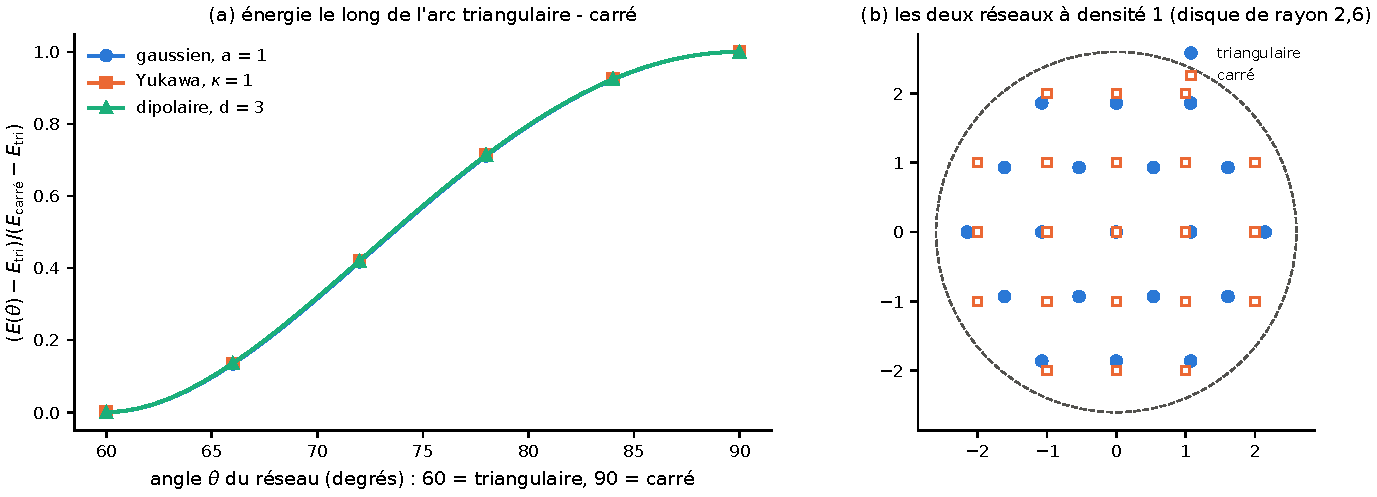
\includegraphics[width=\textwidth]{appF_lattice_energies.pdf}
\caption{Example~2 \tierX. (a) Energy along the lattices of shape $\tau=e^{i\theta}$, normalised between the triangular
($\theta=60^\circ$) and the square ($\theta=90^\circ$) lattice, for the three potentials. (b) The two lattices of
covolume~1.}
\label{appF:fig:energies}
\end{figure}

\begin{exercise}[Example 2]\label{appF:exo2}
(a) Replace \texttt{"gauss"} by a Gaussian $e^{-\pi ar^2}$ with arbitrary parameter $a$, and check on a grid of values of
$a$ that $\Theta_\Lat(a)\le\Theta_{\Z^2}(a)$ (Montgomery's theorem~\cite{app:montgomery}, \tierL). (b) For a potential that is \emph{not}
completely monotone, for instance $V=e^{-r^2}-\tfrac12e^{-r^2/4}$, plot the energy along the same arc. Is the minimum
still at $60^\circ$? What can one conclude from this, and what can one not conclude?
\end{exercise}

% =====================================================================================================
\section[Example 3 -- Complete monotonicity]{Example 3 -- Complete monotonicity: what a computer can say}\label{appF:ex3}

\paragraph{The question.} A function $g$ is completely monotone (CM) if $(-1)^ng^{(n)}(t)\ge0$ for all $n$ and all
$t>0$. A program tests only finitely many pairs $(n,t)$. It can therefore \emph{refute} complete monotonicity, since a
single wrong sign suffices, but never prove it: the proof belongs to the CM/Bernstein library and to the theorem
\lean{ALEXIS} of Chapter~5. What do we see on three CM potentials and on two functions that are not CM?

\paragraph{The code.} \texttt{mpmath.diff} differentiates numerically with 40 significant digits, enough for order~8:
\lstinputlisting[language=Python,style=appFcode,firstline=22,lastline=40,firstnumber=22]{code/examples/python/f03_cm_signs.py}
\appFsortie{f03_cm_signs.txt}

\paragraph{Reading the output.} The three physical potentials pass the $9\times7$ tests. The two counterexamples fail,
and the output says where:
\begin{itemize}
\item $e^{-t}-\tfrac12e^{-2t}$ is a mixture of exponentials whose Bernstein measure $\delta_1-\tfrac12\delta_2$ changes
sign. It fails from $n=2$ on, since $(-1)^ng^{(n)}=e^{-t}-2^{n-1}e^{-2t}<0$ for small $t$.
\item Lennard-Jones fails already at $n=0$: it becomes negative.
\end{itemize}
The first failure is a certificate of non-complete-monotonicity, which can be checked by hand. The successes, for their
part, certify nothing.

\begin{figure}[ht]\centering
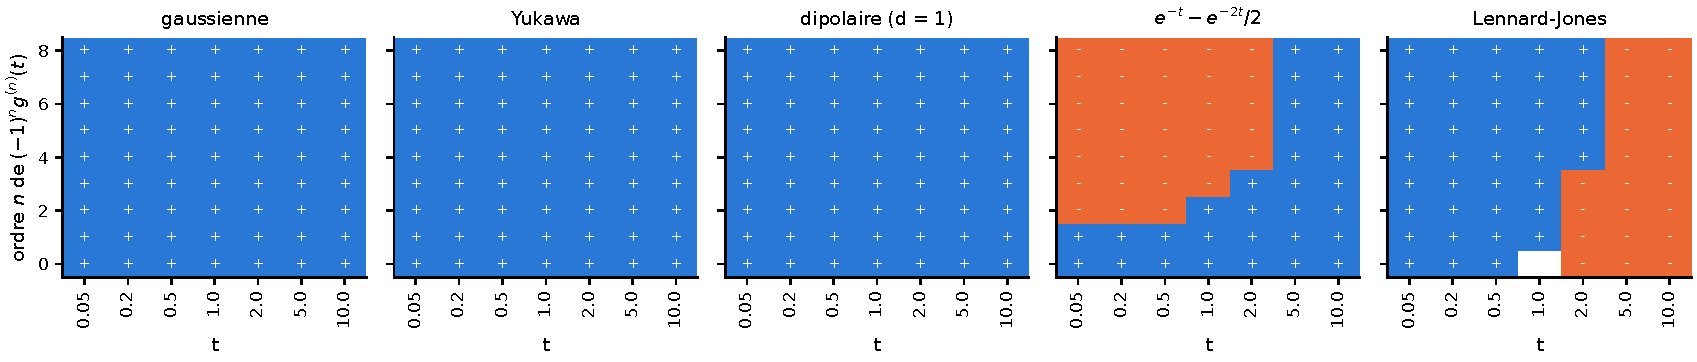
\includegraphics[width=\textwidth]{appF_cm_signs.pdf}
\caption{Example~3 \tierX. Sign of $(-1)^ng^{(n)}(t)$ (blue: $+$, orange: $-$, white: exact zero) for $n\le8$ and seven
values of $t$. The first three potentials are CM (\tierA{} theorems of Chapter~2); the last two are not.}\label{appF:fig:cm}
\end{figure}

\begin{exercise}[Example 3]\label{appF:exo3}
(a) Prove by hand that $e^{-t}-\tfrac12e^{-2t}$ is not CM, starting from the value of $g''(0^+)$. (b) The program says
that $g(t)=e^{-\sqrt t}$ passes all the tests. Prove that it is CM by writing it as $f\circ\phi$, with $f=e^{-s}$ CM and
$\phi=\sqrt{\cdot}$ a Bernstein function (Chapter~1). (c) Add the function $1/(1+t^2)$ to \texttt{FUNCS} and predict,
before running the program, the order $n$ of the first failure.
\end{exercise}

% =====================================================================================================
\section{Example 4 -- Wright--Fisher in exact fractions}\label{appF:ex4}

\paragraph{The question.} In the neutral Wright--Fisher model with $N$ copies of a gene, the next generation is a
binomial draw: $P(i,j)=\binom Nj(i/N)^j(1-i/N)^{N-j}$. The theorem \lean{KAL} (Kolmogorov absorption, \tierA) states
that $P^n(i,N)\to h(i)$ for every harmonic function $h$ with $h(0)=0$ and $h(N)=1$ (and a variance condition). Here
$h(i)=i/N$. Can we see this \emph{exactly}, without rounding? How fast does the convergence take place?

\paragraph{The code.} Python's \texttt{fractions} module computes with exact rationals:
\lstinputlisting[language=Python,style=appFcode,firstline=22,lastline=32,firstnumber=22]{code/examples/python/f04_wright_fisher.py}
\appFsortie{f04_wright_fisher.txt}

\paragraph{Reading the output.} Two equalities are \emph{exact}, not merely to within $10^{-16}$: the matrix is
stochastic and $Ph=h$. With selection ($r=2$), $h(i)=i/N$ is no longer harmonic: this is the negative control. The
denominators grow fast, with 152 digits at $n=60$. The ratio of two successive discrepancies equals
$0.833333333333=1-1/N$, that is, the second eigenvalue of the Wright--Fisher matrix, $\lambda_2=1-1/N$.

\begin{figure}[ht]\centering
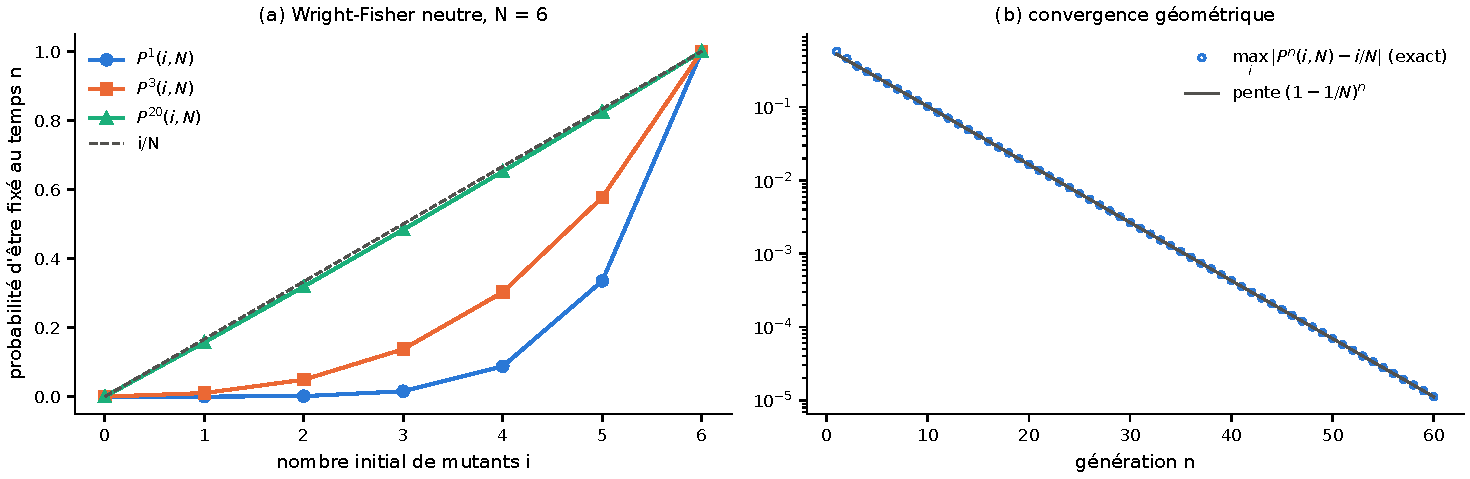
\includegraphics[width=\textwidth]{appF_wright_fisher.pdf}
\caption{Example~4 \tierX. (a) $P^n(i,N)$ for $n=1$, $3$ and $20$, and the limit $i/N$, for $N=6$. (b) The maximal discrepancy,
computed exactly and then converted to floating point, decreases like $(1-1/N)^n$.}\label{appF:fig:wf}
\end{figure}

\begin{exercise}[Example 4]\label{appF:exo4}
(a) Prove that $\lambda_2=1-1/N$ is an eigenvalue of $P$. Hint: apply $P$ to the polynomial $i(N-i)$, after computing
$\mathbb E[X(N-X)]$ for a binomial $X$. (b) Deduce that $|P^n(i,N)-i/N|\le C(1-1/N)^n$. (c) Modify the script for Moran
instead of Wright--Fisher, and compare the rates for equal $N$.
\end{exercise}

% =====================================================================================================
\section{Example 5 -- Isothermal graph versus star}\label{appF:ex5}

\paragraph{The question.} A mutant of fitness $r$ is placed on a vertex of a graph, and the population evolves by
birth--death (the model of N4, Chapter~4). The isothermal theorem \lean{ILENE} (\tierA) states the following: if the
replacement matrix is doubly stochastic, the fixation probability is Moran's, $(1-r^{-1})/(1-r^{-n})$, \emph{whatever}
the starting vertex. What happens on the star, which is not isothermal?

\paragraph{The code.} The state is the set $S$ of mutants, encoded by a bit mask, which gives $2^n$ states. The fixation
probabilities solve a linear system, which we solve in fractions by Gaussian elimination:
\lstinputlisting[language=Python,style=appFcode,firstline=37,lastline=48,firstnumber=37]{code/examples/python/f05_graph_fixation.py}
\lstinputlisting[language=Python,style=appFcode,firstline=51,lastline=76,firstnumber=51]{code/examples/python/f05_graph_fixation.py}
\appFsortie{f05_graph_fixation.txt}

\paragraph{Reading the output.} On the cycle with 4 vertices, which is isothermal, the value is $8/15$ everywhere: it is
Moran's. On the star with 3 vertices we recover the values of N4, all three \tierA{}:
\begin{itemize}
\item $5/12$ for a mutant at the centre;
\item $2/3$ for a mutant on a leaf;
\item $7/12$ for a uniform start, against $4/7$ for Moran.
\end{itemize}
The values of the star with 4 vertices, $392/1265$, $168/253$ and $728/1265$, are only \tierX{} in N4: they come from
an unverified script, and are recovered here by a second script. The last two lines show why the number of mutants is
not a Markov chain on the cycle. With two mutants, the probability of moving up one step is $1/3$ if they are
neighbours and $2/3$ if they are opposite. But the ratio $P^+/P^-$ equals $r=2$ in both cases: this is the
per-configuration bias that N4 proves.

\begin{figure}[ht]\centering
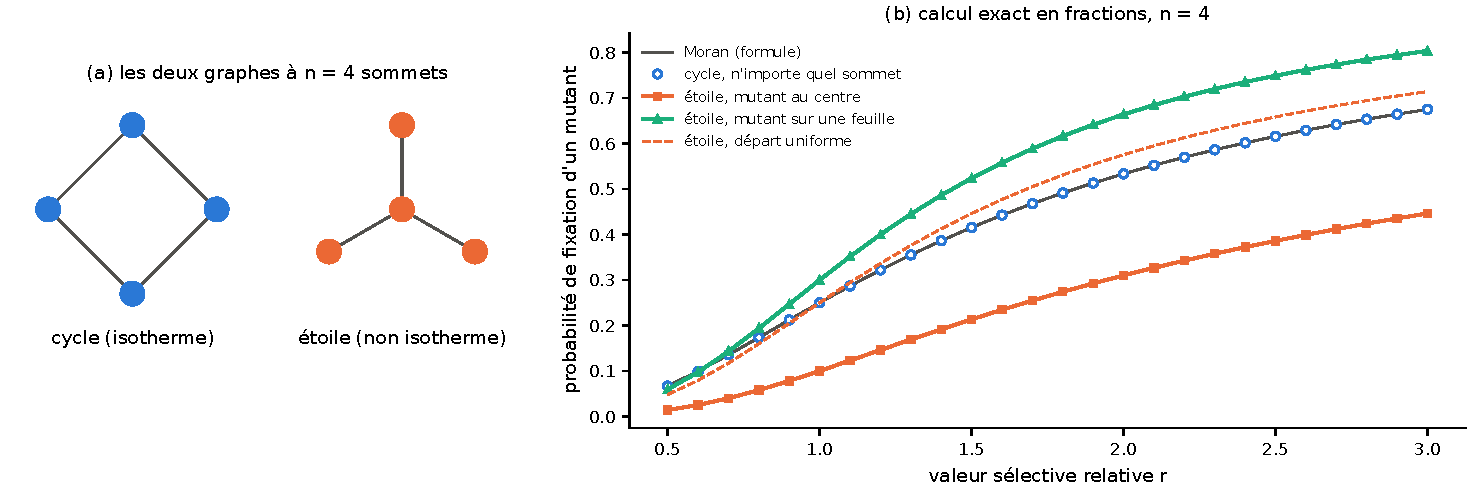
\includegraphics[width=\textwidth]{appF_graph_fixation.pdf}
\caption{Example~5 \tierX, exact computation. (a) The cycle and the star with 4 vertices. (b) Fixation probability of a mutant
as a function of $r$. The cycle follows Moran whatever the vertex. On the star, a mutant at the centre is disadvantaged
and a mutant on a leaf advantaged; on average, the star amplifies selection for $r>1$ in this sample of values.}
\label{appF:fig:graph}
\end{figure}

\begin{exercise}[Example 5]\label{appF:exo5}
(a) Check by hand that, on the star with 3 vertices and $r=2$, the state \texttt{001} (mutant at the centre) moves to
\texttt{011} and to \texttt{101} with probability $1/4$ each, and to the empty state with probability $1/2$. (b) Write
the complete graph $K_4$ (with $W(i,j)=1/3$ for $i\ne j$) and predict the result before running the program. (c) For
the star with $n$ vertices, conjecture the limit of the mean probability as $n\to\infty$, then compare with the
literature (Lieberman, Hauert and Nowak, 2005~\cite{app:lhn}). A conjecture drawn from a few exact values is Tier~X.
\end{exercise}

% =====================================================================================================
\section{Example 6 -- Phonons and zero-point energy}\label{appF:ex6}

\paragraph{The question.} In Chapter~3, conjecture QU-1 asked whether the triangular lattice also minimises the harmonic
zero-point energy $E_{zp}=\tfrac12\langle\omega_1+\omega_2\rangle_{\mathrm{ZB}}$. For the Gaussian $e^{-\pi ar^2}$, the
P2 programme found the opposite (\tierX). On $a\in(0.37668, 1.58148)$, the triangular lattice is a local
\emph{maximum} of $E_{zp}$. Can we recover this with thirty lines of numpy?

\paragraph{The code.} The dynamical matrix $D(\mathbf k)=\sum_{R\ne0}(1-\cos\mathbf k\cdot R)\,\mathrm{Hess}\,V(R)$ is
$2\times2$, so its eigenvalues have a closed form. The average over the Brillouin zone is taken on an $n\times n$ grid
of the reciprocal cell. The fractional grid is the same for all shapes $\tau$, which makes the grid error cancel in the
differences:
\lstinputlisting[language=Python,style=appFcode,firstline=41,lastline=67,firstnumber=41]{code/examples/python/f06_phonons_zero_point.py}
\appFsortie{f06_phonons_zero_point.txt}

\paragraph{Reading the output.} The positive controls are the P2 values. For $a=1$, the script recovers
$E_{zp}(\rho)=1.5033523522$ to within $3\times10^{-8}$ on the grid $n=192$. It also recovers P2's counterexample, the
rhombus $\tau=0.5+0.966025\,i$, lower by $1.3074\times10^{-2}$. The curvature $c(a)$ changes sign as announced:
\begin{itemize}
\item it is negative for $a=0.5$ and $a=1$, where $\rho$ is a local maximum;
\item it is positive for $a=0.25$ and $a=2$, where $\rho$ is a local minimum.
\end{itemize}
The four P2 values are recovered to within one thousandth, and the curvature does not move between grids $48$ and
$96$. All of this remains \tierX: it is a second floating-point computation, not a proof. The B2 certificate of
Chapter~3 treats the case $a=1$ with ball arithmetic.

\begin{figure}[ht]\centering
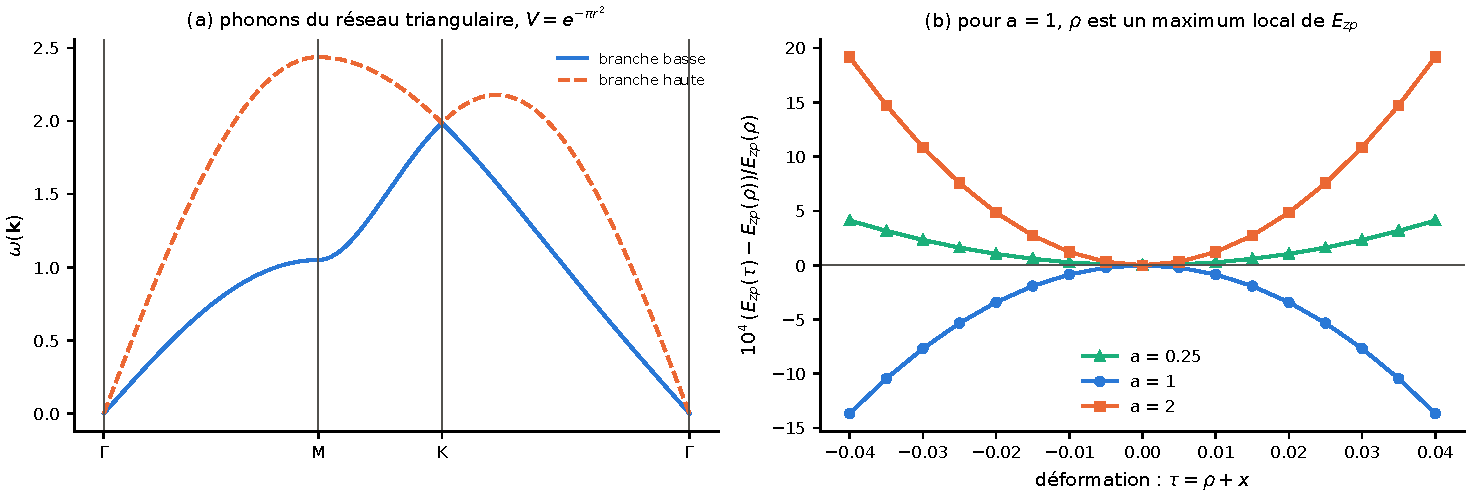
\includegraphics[width=\textwidth]{appF_phonons.pdf}
\caption{Example~6 \tierX. (a) The two phonon branches of the triangular lattice for $V=e^{-\pi r^2}$, along
$\Gamma$--M--K--$\Gamma$; they vanish at $\Gamma$, as for every crystal (acoustic modes). (b) Relative variation of
$E_{zp}$ when $\rho$ is deformed into $\rho+x$: a downward parabola for $a=1$ (local maximum), upward for $a=0.25$ and
$a=2$.}\label{appF:fig:phonons}
\end{figure}

\begin{exercise}[Example 6]\label{appF:exo6}
(a) Prove that $D(\mathbf k)$ is symmetric and that $D(\mathbf 0)=0$. Why is $\omega(\mathbf k)$ linear in
$|\mathbf k|$ near $\Gamma$? (b) Modify \texttt{curvature} to plot $c(a)$ on $a\in[0.3, 1.7]$ and locate numerically
the two sign changes (P2: $0.37668$ and $1.58148$). (c) Why can the statement ``the triangular lattice is a local
maximum of $E_{zp}$ for $a=1$'' not become Tier~A with this code alone?
\end{exercise}

% =====================================================================================================
\section[Example 7 -- CVODE in Rust]{Example 7 -- CVODE in Rust: a stiff ODE, then the Kolmogorov equation}\label{appF:ex7}

\paragraph{The question.} rusty-SUNDIALS is a Rust rewrite of SUNDIALS. Its CVODE solver integrates stiff differential
equations with the BDF formulas. How is it called from an independent crate? And why does an explicit scheme fail where
BDF succeeds?

\paragraph{A stiff ODE.} The Prothero--Robinson problem, $y'=\lambda(y-\cos t)-\sin t$ with $y(0)=2$ and
$\lambda=-10^4$, has the exact solution $y=\cos t+e^{\lambda t}$. Here is the call to CVODE (a function of the crate's
library):
\lstinputlisting[language=Rust,style=appFcode,firstline=36,lastline=68,firstnumber=36]{code/examples/rust/src/lib.rs}
\appFsortie{f07a_tb_stiff.txt}

\paragraph{Reading the output.} CVODE follows the exact solution to within $6\times10^{-9}$ during the transient phase,
where $e^{\lambda t}$ dies out within $10^{-4}$, then to within $3\times10^{-11}$ up to $t=10$. It gets there in 506
steps. The explicit Euler scheme is stable only if $|1+h\lambda|\le1$, that is, $h\le2/|\lambda|=2\times10^{-4}$:
\begin{itemize}
\item with $h=10^{-4}$ it succeeds, but in $10\,000$ steps;
\item with $h=2.5\times10^{-4}$, the error is multiplied by $|1+h\lambda|=1.5$ at each step, reaches $4\times10^{17}$
in 100 steps and ends in \texttt{NaN}.
\end{itemize}
This is the negative control, and the very definition of stiffness.

\begin{uniremark}\tierL{} The BDF formulas of orders~1 and~2 are A-stable: their stability region contains the whole
left half-plane, so they accept any step $h>0$ on $y'=\lambda y$ with $\operatorname{Re}\lambda<0$. By Dahlquist's
second barrier, no A-stable linear multistep method has order greater than~2; the higher-order BDF formulas used by CVODE
(up to order~5) are only $A(\alpha)$-stable, with a stability sector that narrows as the order grows. CVODE varies both the step
size and the order (1 to 5) during an integration~\cite{app:sundials} (standard).\end{uniremark}

\paragraph{Moran's Kolmogorov equation.} The Moran chain (Chapter~4), uniformised in continuous time, obeys
$\dot\pi=\pi(P-I)$. The mass absorbed at $N$ tends to the fixation probability $\varphi_i=(1-r^{-i})/(1-r^{-N})$. The
Jacobian is the constant matrix $(P-I)^{\mathsf T}$. We double the output time until the interior mass falls below
$10^{-12}$:
\lstinputlisting[language=Rust,style=appFcode,firstline=125,lastline=172,firstnumber=125]{code/examples/rust/src/lib.rs}
\appFsortie{f07b_tb_moran_forward.txt}

\paragraph{Reading the output.} For $N=3$, $r=2$ and $i=1$, CVODE gives $4/7$ to within $9.5\times10^{-14}$. For
$N=10$, the 27 values ($r=0.8$, $1$ and $1.5$, $i=1,\dots,9$) follow the formula to within $10^{-12}$. The two negative
controls are refused:
\begin{itemize}
\item the identity kernel, which never absorbs;
\item the formula with the inverted exponent, which gives $1/7$.
\end{itemize}
The \texttt{qf-popgen} crate of Chapter~5 does the same computation with a more complete absorption certificate. It is
not yet merged into \texttt{main}, which is why this crate rewrites the equation directly.

\begin{figure}[ht]\centering
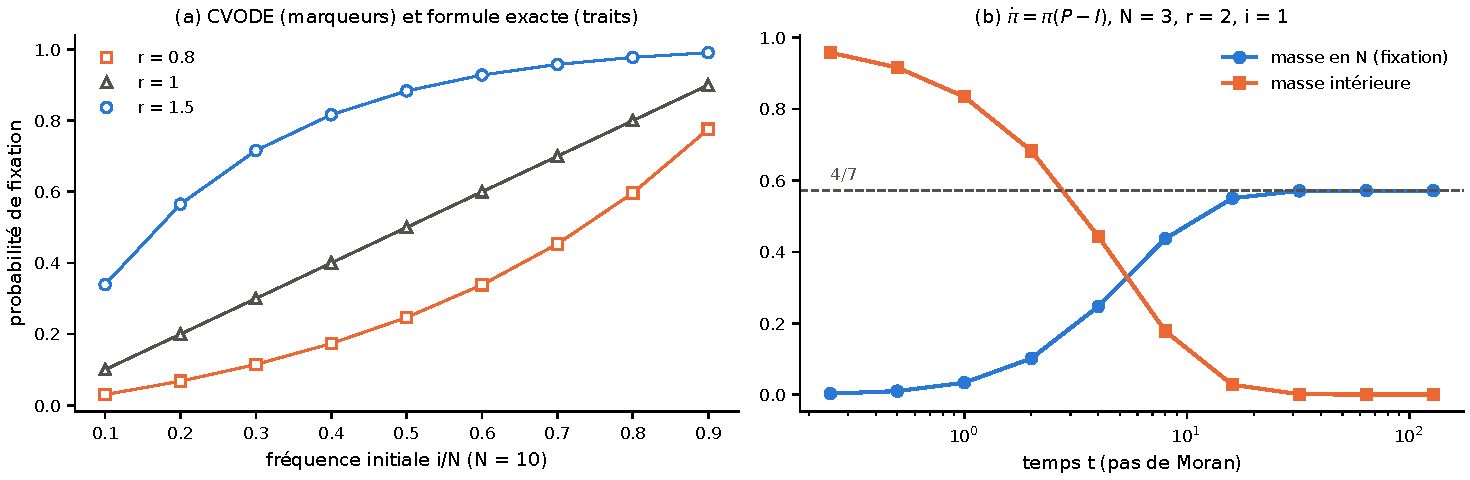
\includegraphics[width=\textwidth]{appF_rust_moran.pdf}
\caption{Example~7 \tierX, plotted from the CSV files written by \texttt{tb\_moran\_forward}. (a) Fixation probability
for $N=10$: CVODE (markers) and exact formula (lines). (b) $N=3$, $r=2$, $i=1$: the mass at $N$ rises towards $4/7$ and
the interior mass dies out, at the output times $0.25\cdot2^k$.}\label{appF:fig:moran}
\end{figure}

\begin{exercise}[Example 7]\label{appF:exo7}
(a) For $y'=\lambda y$, show that the implicit Euler scheme (BDF of order~1) gives $y_{n+1}=y_n/(1-h\lambda)$, which is
stable for every $h>0$ if $\lambda<0$. (b) Why does the interior mass decay exponentially, and what rate should be
expected for $N=3$, $r=2$? Compute the eigenvalues of the restriction of $P-I$ to the interior states. (c) Add a
control: a kernel one of whose rows sums to $1.001$. Which quantity computed by \texttt{absorb} detects it?
\end{exercise}

% =====================================================================================================
\section{Example 8 -- Relaxing a small Yukawa crystal}\label{appF:ex8}

\paragraph{The question.} 64 particles interact via $e^{-2r}/r$ in a periodic box. If they are released from an
arbitrary position and descend the energy gradient ($\dot x=F(x)$), do they recover the triangular lattice? The theorem
says only that the triangular lattice is the \emph{global minimum} (\tierA, conditional). It does not say that the
descent reaches it.

\paragraph{The code.} The crate calls the API of \texttt{qf-yukawa-crystal}:
\begin{itemize}
\item \texttt{ExactBox} for the energy, the forces and the Hessian summed over the images up to $R=12$;
\item \texttt{lattice\_energy\_exact} for the exact energy of the lattice.
\end{itemize}
The relaxation itself is a CVODE integration whose Jacobian is minus the Hessian (function \texttt{relax\_traced} of the
library). Here is the main program:
\lstinputlisting[language=Rust,style=appFcode,firstline=60,lastline=105,firstnumber=60]{code/examples/rust/src/bin/tb_yukawa_relax.rs}
\appFsortie{f08_tb_yukawa_relax.txt}

\paragraph{Reading the output.} The three starts behave as expected.
\begin{itemize}
\item \emph{Perturbed triangular lattice} (positive control): it returns to the exact lattice energy, to within
$10^{-16}$. This energy, $0.393542848871227$ at $R=12$, differs by $6\times10^{-11}$ from the value at $R=20$ recorded in
\texttt{exact\_refs.jsonl}, which is $0.39354284893239$; this is the omitted tail.
\item \emph{Random start}: it stops $2.1\times10^{-3}$ \emph{above}, at a stationary point (forces below $10^{-9}$) that
has defects (Figure~\ref{appF:fig:yukawa}b). We did not check the Hessian: nothing here says that it is a local
minimum. A gradient descent does not always find the global minimum.
\item \emph{Square lattice in a square box} (negative control): it descends below the energy of the square lattice,
which indicates that the square lattice is not a minimum, but it remains above the triangular lattice, which the
$8\times8$ box cannot contain.
\end{itemize}

\begin{figure}[ht]\centering
\includegraphics[width=\textwidth]{appF_rust_yukawa.pdf}
\caption{Example~8 \tierX. (a) Energy per particle above the triangular lattice during the CVODE relaxation, at the
output times $0.01\cdot2^k$. (b) Final state of the random start: triangular domains and defects. (c) Final state in the
square box.}\label{appF:fig:yukawa}
\end{figure}

\begin{exercise}[Example 8]\label{appF:exo8}
(a) Why can the box $8a\times4\sqrt3\,a$ contain exactly the $8\times8$ triangular lattice of spacing $a$, whereas the
$8\times8$ box cannot? (b) Change the seed of the random start (11) to five other values. How many starts reach the
triangular lattice to within $10^{-10}$? (c) Does this result contradict the theorem?
\end{exercise}

% =====================================================================================================
\section{Example 9 -- The invariants of the \texorpdfstring{$\sigma=3$}{sigma=3} shell model}\label{appF:ex9}

\paragraph{The question.} The shell model of Section~\ref{ch5:U4} conserves two quantities:
\begin{itemize}
\item $S=\sum|v_n|^2$;
\item $H_3$, whose quadratic part equals $2D\Omega$, where $\Omega$ is the enstrophy.
\end{itemize}
Lean deduces from them the bound $2D\,\Omega(t)\le H_3(0)+S(0)^{3/2}$ along solutions (\tierAs, Chapter~5). Does a
numerical integrator conserve these invariants? And does the bound hold along a trajectory?

\paragraph{The code.} Six shells, $D=0.05$, integration up to $T=2$ with \texttt{integrate\_cvode} of
\texttt{qf-shell-cascade}, which evaluates the invariants at each internal CVODE step. The negative control multiplies
one coupling by $1+10^{-2}$:
\lstinputlisting[language=Rust,style=appFcode,firstline=18,lastline=63,firstnumber=18]{code/examples/rust/src/bin/tb_shell_sigma3.rs}
\appFsortie{f09_tb_shell_sigma3.txt}

\paragraph{Reading the output.} For the exact model, the invariants drift by $5\times10^{-10}$ for $S$ and by
$9\times10^{-8}$ for $H_3$, relative to the scale of its terms. These drifts come from the solver tolerance, not from
the model. The Lean bound is far from attained, with a maximal ratio of $0.29$. With the perturbed coupling, the drifts
rise to $3$ and $4\times10^{-3}$: conservation rests on the exact cancellation of the nonlinear terms, which the negative
control breaks. We restrict ourselves to six shells: the fastest rotation, $\omega_n=Dk_n^3$ with $k_n=2^n$, is
multiplied by~8 with each added shell, and CVODE must resolve it step by step.

\begin{figure}[ht]\centering
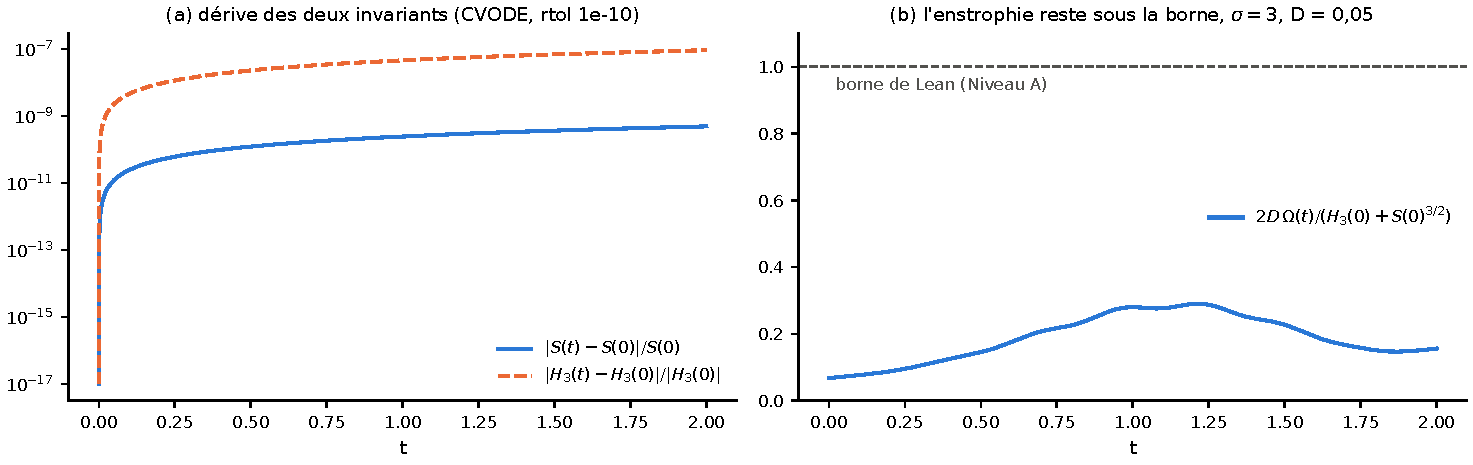
\includegraphics[width=\textwidth]{appF_rust_shell.pdf}
\caption{Example~9 \tierX, plotted from the CSV written by \texttt{tb\_shell\_sigma3} (one internal step in twenty).
(a) Relative drift of the two invariants. (b) The ratio $2D\Omega(t)/(H_3(0)+S(0)^{3/2})$ stays below~1, as the Lean
theorem requires.}\label{appF:fig:shell}
\end{figure}

\begin{exercise}[Example 9]\label{appF:exo9}
(a) Prove that $\frac{d}{dt}\sum|v_n|^2=0$ for the model without dissipation. Group the coupling terms in pairs.
(b) Replace \texttt{sigma: 3.0} by \texttt{2.0}. Are the invariants $S$ and $H_2$ still conserved? Why does the
enstrophy bound no longer follow in the same way?
\end{exercise}

% =====================================================================================================
\section[Example 10 -- LeanFlow]{Example 10 -- LeanFlow: certifying fractions, rejecting a lie}\label{appF:ex10}

\paragraph{The question.} Example~\ref{appF:ex5} computed in Python the exact table of fixation probabilities of the
star with 3 vertices. Python can make mistakes, or be badly programmed. How can these fractions be checked by the Lean
kernel, without writing a single line of Lean?

\paragraph{The code.} LeanFlow's \texttt{lean.certify} receives claims about rationals. It translates them into
statements about integers, has them decided by \lean{decide +kernel} (tactic \texttt{decide\_kernel}), then audits
\texttt{\#print axioms}. An exact Python oracle must return the same verdict as the kernel; otherwise the result is an
error, never a success. Here is the construction of the claim ``the table $x_S$ is harmonic'':
\lstinputlisting[language=Python,style=appFcode,firstline=34,lastline=49,firstnumber=34]{code/examples/python/f10_leanflow_certify.py}
\appFsortie{f10_leanflow_certify.txt}
Here is the shorter of the two generated certificates, as the kernel decided it:
\lstinputlisting[language=Lean,style=appFcode]{code/examples/lean/f10_generated_PosMeanAboveMoran.lean}

\paragraph{Reading the output.} The two true claims are accepted:
\begin{itemize}
\item the six first-step equations, satisfied exactly by the table $(0,\tfrac5{12},\tfrac23,\tfrac56,
\tfrac23,\tfrac56,\tfrac{14}{15},1)$;
\item the inequality $7/12>4/7$.
\end{itemize}
The two planted claims are rejected, with \lean{sorryAx} in the list of axioms:
\begin{itemize}
\item the Moran vector $(0,\tfrac47,\tfrac67,1)$ indexed by $|S|$ violates the six interior equations, but it satisfies
the two boundary conditions (\texttt{cert\_0} and \texttt{cert\_1} are not refused);
\item the reversed inequality $7/12<4/7$ is refused.
\end{itemize}
LeanFlow checks only \texttt{\#print axioms}, which can be fooled (Chapter~2). The script therefore completes the Tier~A
gate. Each accepted source is recompiled to \texttt{.olean} with Lean~4.34.1 and then replayed by \texttt{leanchecker},
with exit code~0 for both. None of the words \texttt{skipKernelTC}, \texttt{addDecl}, \texttt{native\_decide} or
\texttt{implemented\_by} occurs in them. The replay control, a nonexistent module, exits with code~1. The two
certificates are therefore \tierA, but for the \emph{arithmetic statement only}. That this table is the fixation
probability of the star requires in addition the uniqueness of the harmonic solution (Chapter~4) and the identification
of the Python transitions with those of \lean{bdK}. This link is a human argument, \tierC.

\begin{exercise}[Example 10, LeanFlow]\label{appF:exo10}
(a) Certify in the same way the table of the cycle with 4 vertices ($2^4$ states, value $8/15$ for every single
mutant). (b) Plant a one-ulp error: replace $5/12$ by the fraction of the float \texttt{float(5/12)}. Does LeanFlow
accept it? Why is a certificate on rationals more demanding than a floating-point comparison to within $10^{-15}$?
\end{exercise}

% =====================================================================================================
\section{Example 11 -- Reading and checking the theorem ILENE}\label{appF:ex11}

\paragraph{The question.} Chapter~5 cites \lean{ILENE}, the single-mutant version of the isothermal theorem. How can the
reader see, on their own machine, the exact statement that Lean checked and the axioms its proof depends on? And how
can a real proof be told apart from a fake one?

\paragraph{The code.} A 21-line file, of which we reproduce lines 2 to 21, imports the compiled module and asks Lean four questions:
\lstinputlisting[language=Lean,style=appFcode,firstline=2,firstnumber=2]{code/examples/lean/f11_ilene.lean}
(The first line of the file, the \texttt{import} of the acronym module, is omitted here.)
It is compiled with Lean~4.34.1 and Mathlib \texttt{d13f23b7}, through the script \texttt{lean\_pinned.py} of the
directory \texttt{scripts/certified\_numerics/}. It gives:
\appFsortie{f11_ilene.txt}

\paragraph{Reading the output.} The output is read in four steps.
\begin{itemize}
\item \texttt{\#check} displays the full statement. The hypotheses are: $0<n$, $0<r$, $r\ne1$, $W$ isothermal and
strongly connected. The conclusion is a limit, that of $P^t(\{v\},V)$ to $(1-r^{-1})/(1-r^{-n})$, for every vertex $v$.
\item The axioms are exactly those of the whitelist. The acronyms module and its sources were replayed by
\texttt{leanchecker}, with exit code~0 (record \texttt{acronymes\_leanchecker.json}): \lean{ILENE} is therefore \tierA.
\item The \texttt{example} checks, by \lean{norm_num}, that the limit value equals $8/15$ for $n=4$ and $r=2$. This is
the value of the cycle of Example~\ref{appF:ex5}.
\item The planted witness asserts a false value, $4/7$, ``proved'' by \lean{sorry}. The file compiles all the same, with
exit code~0 and a mere warning. Only the \texttt{\#print axioms} line betrays the fraud: it displays \lean{sorryAx}.
\end{itemize}
This is the lesson of Chapter~2: a zero exit code proves nothing; one must read the axioms and replay the kernel.

\begin{exercise}[Example 11, Lean]\label{appF:exo11}
(a) Add \texttt{\#check @KAL} and \texttt{\#print axioms AURELIA}, and reread the statements with the help of the table
of acronyms (Section~\ref{ch5:acronymes}). (b) Replace \lean{by sorry} by \lean{by norm_num} in the planted witness.
What does Lean answer, and with which exit code? (c) Why is the equality $1/2=2^{-1}$, used implicitly when comparing
the \texttt{example} with the statement of \lean{ILENE}, a link to be checked, and how can this be done in Lean?
\end{exercise}

% =====================================================================================================
\section{Example 12 -- Cross-check: CVODE versus SciPy}\label{appF:ex12}

\paragraph{The question.} Two codes written by the same team can share the same error. Are the numbers of
Example~\ref{appF:ex7} confirmed by \emph{independent} methods?

\paragraph{The code.} The script rereads the outputs of the Rust binary and recomputes the same quantities in two ways:
\begin{itemize}
\item for the stiff problem, with SciPy's Radau method, an implicit Runge--Kutta method and not BDF;
\item for Moran, with the matrix exponential $\pi(t)=e_i\,e^{t(P-I)}$, without any time step.
\end{itemize}
\lstinputlisting[language=Python,style=appFcode,firstline=56,lastline=78,firstnumber=56]{code/examples/python/f12_scipy_crosscheck.py}
\appFsortie{f12_scipy_crosscheck.txt}

\paragraph{Reading the output.} After the transient phase, CVODE and Radau agree to within $3\times10^{-11}$. At the
first two instants, the discrepancy of $5\times10^{-9}$ is that of CVODE from the exact solution: the Radau value
coincides with $\cos t+e^{\lambda t}$, and the CVODE tolerance was $10^{-8}$. For Moran, CVODE and the matrix exponential
agree to within $1.3\times10^{-11}$ at the ten output times. The negative control shifts one time by $10^{-3}$, and the
discrepancy, of $8\times10^{-4}$, becomes immediately visible: the comparison therefore has the power to detect an
error.

\begin{exercise}[Example 12]\label{appF:exo12}
(a) Replace \texttt{method="Radau"} by \texttt{"RK45"}, an explicit method. How many evaluations are needed, and why?
(b) For Moran, the matrix exponential is exact up to rounding. Why does it not replace CVODE for $N=1000$?
\end{exercise}

% =====================================================================================================
\section{Summary}\label{appF:bilan}

The twelve examples were run on 2026-10-26, and all their controls behaved as expected. They illustrate the three ways
of handling a number in this book.
\begin{itemize}
\item \emph{Floating-point computation} (Examples~1, 2, 3, 6 to 9 and 12) explores, checks and refutes. It recovers the
published values to the expected precision, but it remains Tier~X.
\item \emph{Exact rational computation} (Examples~4 and~5) removes rounding, but not the risk of a programming error.
\item \emph{The Lean kernel} (Examples~10 and~11) removes that risk for the checked statement, and for it alone. The link
between that statement and the question asked remains a link to be checked separately.
\end{itemize}
